\documentclass[11pt,a4paper]{article}
\usepackage[utf8]{inputenc}
\usepackage[spanish]{babel}	%Idioma
\usepackage{amsmath}
\usepackage{amsfonts}
\usepackage{amssymb}
\usepackage[document]{ragged2e}

\usepackage{graphicx} %Añadir imágenes
\graphicspath{{img/}}

\usepackage{geometry}	%Ajustar márgenes
\usepackage[export]{adjustbox}[2011/08/13]
\usepackage{float}
\restylefloat{table}
\usepackage{fontspec}
\usepackage{hyperref}
\usepackage{titling}
\usepackage[font=small,labelfont=bf]{caption} 

%Opciones de encabezado y pie de página:
\usepackage{fancyhdr}
\pagestyle{fancy}
\lhead{}
%\rhead{}
\lfoot{Servidores Web de Altas Prestaciones}
\cfoot{}
\rfoot{\thepage}
\renewcommand{\headrulewidth}{0.4pt}
\renewcommand{\footrulewidth}{0.4pt}
%Opciones de fuente:
\usepackage[utf8]{inputenc}
%\usepackage[default]{sourcesanspro}
%\usepackage{sourcecodepro}
\usepackage[T1]{fontenc}

\setmainfont [ 
Path = /usr/share/fonts/liberation/, 
UprightFont = *-regular,
BoldFont = *-bold,
ItalicFont = *-italic] {LiberationSans}

\setmonofont [
Path = /usr/share/fonts/TTF/,
UprightFont = Hack-Regular
] {Hack}

\setlength{\parindent}{0pt}
\setlength{\headheight}{15pt}
\setlength{\voffset}{10mm}

% Custom colors
\usepackage{color}
\definecolor{deepblue}{rgb}{0,0,0.5}
\definecolor{deepred}{rgb}{0.6,0,0}
\definecolor{deepgreen}{rgb}{0,0.5,0}

\usepackage{listings}

% Evitar guiones al final de línea.
\tolerance=1
\emergencystretch=\maxdimen
\hyphenpenalty=10000
\hbadness=10000

\pretitle{%
  \centering
  \LARGE
  
\includegraphics[scale=0.6]{logo.png}\\[\bigskipamount]
}
\posttitle{\begin{center} \end{center}}

\author{Juan Ocaña Valenzuela}
\title{\textbf{Servidores Web de Altas Prestaciones} \\ 
 \textbf{Trabajo \#35:} Configuración de VPN en máquinas virtuales o Raspberry Pi para asegurar una granja web.}

%%%%%%%%%%%%%%%%%%%%%%%%%%%%%%%%%%%%%%%%%%%%%%%%%%%%%%%%%%%%%%%%%%%%%%%%%%%%%%%
%% EL DOCUMENTO EMPIEZA AQUÍ
%%%%%%%%%%%%%%%%%%%%%%%%%%%%%%%%%%%%%%%%%%%%%%%%%%%%%%%%%%%%%%%%%%%%%%%%%%%%%%%

\begin{document}

\thispagestyle{empty}

\maketitle

\begin{center}
%\url{https://github.com/patchispatch}

Versión: 1.0
\end{center}

\newpage

\tableofcontents

\newpage

\section{Introducción}

A lo largo de este documento se explorará qué es una VPN (\textit{Virtual Private Network}), cómo construir, configurar y conectar nuestro propio servidor VPN y qué utilidad puede brindar en un centro de datos de diferentes maneras.

\section{Qué es una VPN}

Una \textbf{Red Privada Virtual} o \textbf{VPN} es una tecnología que permite establecer una red local a través de una infraestructura pública a través de un túnel cifrado. De esta forma, se pueden comunicar distintos equipos y servicios de forma distribuida como si estuviesen dentro de la misma red, aun encontrándose repartidos por todo el mundo. 

\medskip

Además, el servidor VPN actúa como intermediario de las conexiones, por lo que, a ojos de internet, nuestra IP pública pasa a ser la del servidor. Las comunicaciones están completamente cifradas, evitando posibles ataques \textit{man in the middle}, y gracias a este tipo de conexiones y una buena configuración de cortafuegos se puede limitar el acceso a una infraestructura a través de internet. 

\medskip

Más adelante veremos distintas posibles aplicaciones de esta tecnología en el ámbito de los centros de datos y las granjas de servidores, pero ahora veremos paso a paso cómo instalar nuestra propia infraestructura VPN ---servidor, entidad certificadora y clientes--- mediante la herramienta \textbf{OpenVPN}.

\section{Instalación de infraestructura VPN mediante OpenVPN}

\subsection{OpenVPN}

OpenVPN es una herramienta y protocolo de código abierto utilizada en todo el mundo para establecer este tipo de conexiones. Su extensa documentación y comunidad activa, así como numerosas guías de instalación y uso, son un punto fuerte por el cual es una opción muy recomendable. Además es multiplataforma, por lo que se pueden configurar servidores y clientes en diferentes sistemas operativos.

\subsection{Antes de instalar}

Inicialmente se iba a realizar la instalación en una Raspberry Pi 3 B+, pero debido a las circunstancias excepcionales es imposible acceder a ella en estos momentos. Sin embargo, el procedimiento es el mismo y no debería haber mayor problema en replicarlo en Raspbian u otros sistemas, salvo ligeras diferencias en el gestor de paquetes y la localización de algunos archivos de configuración.

\subsection{Preparación}

\subsubsection{Servidor VPN}

Para el servidor VPN, utilizaremos una máquina virtual con Ubuntu 18.04 LTS, con 10GB de disco y 1024MB de RAM. Para asegurar que dispone de una IP única, debemos configurar el adaptador sólo-anfitrión de VirtualBox.

\medskip

En el instalador de Ubuntu proporcionamos los siguientes datos:

\begin{itemize}
\item \textbf{Nombre del servidor:} vpn
\item \textbf{Nombre de usuario:} patchispatch
\item \textbf{Contraseña:} Swap1234
\end{itemize}

Es necesario que el usuario creado tenga privilegios \texttt{sudo}, algo que el instalador de Ubuntu hace por nosotros.

Además, le proporcionaremos una IP estática, en este caso \texttt{192.168.56.106} mediante la configuración de netplan:

\begin{lstlisting}[tabsize=4]
network:
	ethernets:
		enp0s3:
			dhcp4: true
		enp0s8:
			addresses:
				- 192.168.56.106/24
	version: 2
\end{lstlisting}

Una vez modificada la configuración, aplicamos los cambios con \texttt{sudo netplan apply}. Ya tenemos nuestra máquina lista para conectarse con el resto de la red local.


\subsubsection{Entidad certificadora}

Aunque es posible utilizar la misma máquina servidora como entidad certificadora, la documentación oficial de OpenVPN recomienda que se utilice una máquina dedicada de forma exclusiva a importar y firmar certificados.

\medskip

Para esta máquina certificadora, utilizaremos también Ubuntu 18.04 LTS, con 10GB de disco y 512MB de RAM. De nuevo, configuramos el adaptador sólo-anfitrión de VirtualBox para permitir que nuestra máquina disponga de una IP única para comunicarse con otras máquinas.

\medskip

En el instalador de Ubuntu proporcionamos los siguientes datos:

\begin{itemize}
\item \textbf{Nombre del servidor:} ca
\item \textbf{Nombre de usuario:} patchispatch
\item \textbf{Contraseña:} Swap1234
\end{itemize}

De nuevo, necesitamos un usuario con privilegios \texttt{sudo}, aunque ya hemos visto que Ubuntu se encarga de ello.

La entidad certificadora tendrá la IP estática \texttt{192.168.56.107}:

\begin{lstlisting}[tabsize=4]
network:
	ethernets:
		enp0s3:
			dhcp4: true
		enp0s8:
			addresses:
				- 192.168.56.107/24
	version: 2
\end{lstlisting}

\subsubsection{Cortafuegos básico}

Para establecer seguridad tanto en el servidor VPN como en la entidad certificadora, vamos a establecer un firewall básico. En lugar de utilizar iptables como se ha visto en la asignatura, usaremos la herramienta **ufw**, dada su facilidad de uso.

Partiremos de una configuración que permita únicamente el acceso mediante SSH en ambas máquinas.

\medskip

\begin{center}
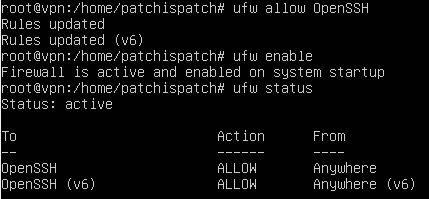
\includegraphics[scale=0.8]{ufw-allow.png}
\end{center}

\subsection{Instalación de servicios}

En primer lugar, instalamos en nuestra máquina \textbf{vpn} el servidor OpenVPN con \texttt{sudo apt install openvpn}.

Para configurar la entidad certificadora, debemos descargar mediante \textit{wget} el paquete \texttt{EasyRSA} con la siguiente orden, \textbf{tanto en la máquina \textit{vpn} como en la máquina \textit{ca}}:

\medskip

\texttt\footnotesize{wget -P $\sim$/ https://github.com/OpenVPN/easy-rsa/releases/download/v3.0.7/EasyRSA-3.0.7.tgz}

\medskip

Y extraemos con \texttt{tar xvf}.

\subsection{Configuración de la entidad certificadora}

Para configurar la entidad certificadora, en nuestra máquina \textbf{CA} entramos en la carpeta \texttt{EasyRSA-3.0.7} que acabamos de descomprimir, y copiamos el archivo \texttt{vars.example} como \texttt{vars} para editarlo. 

Debemos especificar los datos de nuestra entidad certificadora, descomentando los valores del archivo y fijando los que queramos. Los datos de nuestra entidad certificadora serán los siguientes:

\medskip

\begin{center}
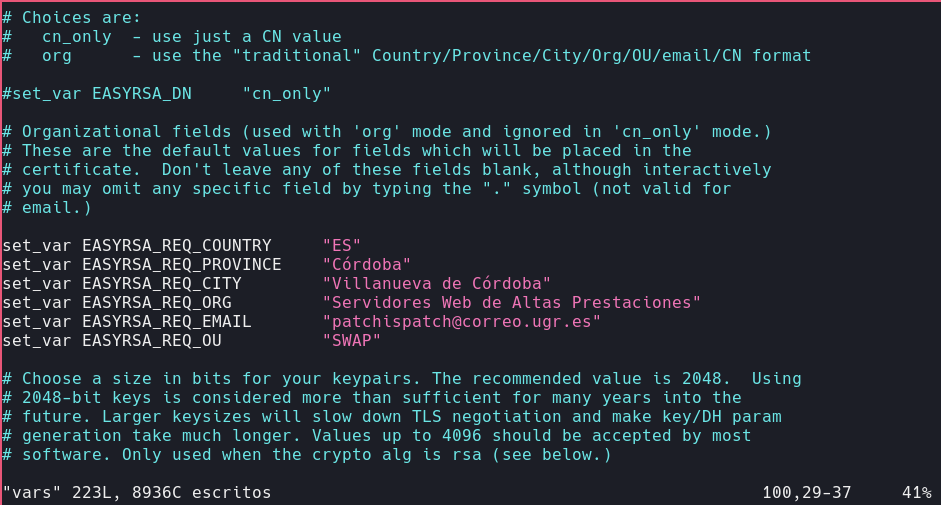
\includegraphics[scale=0.4]{vars.png}
\end{center}

Para gestionar el servicio de RSA, debemos ejecutar el script \texttt{easyrsa} con una serie de opciones. Primero lo ejecutamos con la opción \texttt{init-pki}, para crear la infraestructura de claves públicas. Esto lo realizamos en el servidor \textbf{CA}, no en el servidor VPN.

\medskip

\begin{center}
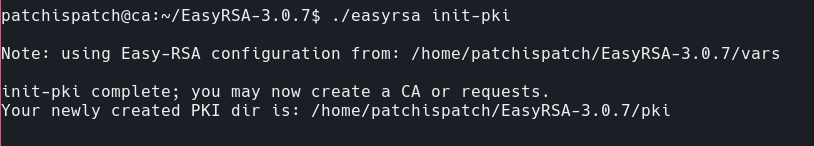
\includegraphics[scale=0.4]{init-pki.png}
\end{center}

\medskip

Para crear el certificado, ejecutamos de nuevo el script \texttt{easyrsa}, esta vez con la opción \texttt{build-ca}. Esto generará los archivos \texttt{ca.crt} y \texttt{ca.key}. Como vamos a generar el certificado sin contraseña esta vez, debemos indicar también la opción \texttt{nopass}:

\medskip

\begin{center}
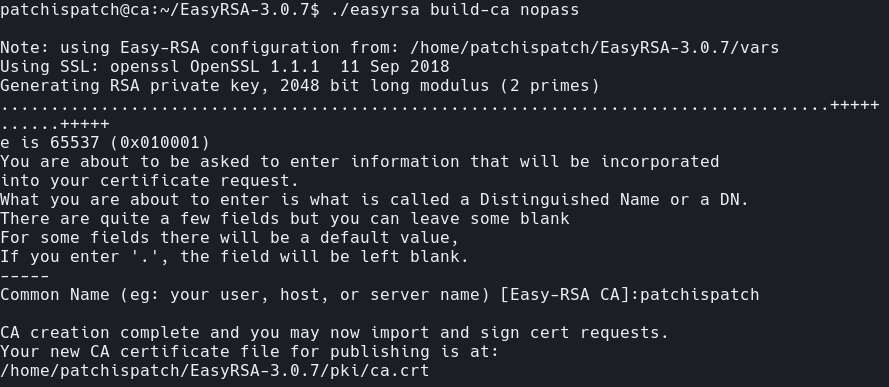
\includegraphics[scale=0.4]{build-ca.png}
\end{center}

\medskip

Con estos pasos, la entidad certificadora está lista para firmar certificados.


\subsection{Generación y firmado del certificado del servidor}

Para generar un certificado para nuestro servidor OpenVPN, debemos abrir la carpeta EasyRSA-3.0.7 en nuestra máquina, e inicializar la infraestructura de claves con \texttt{./easyrsa init-pki}, como hicimos con nuestra entidad certificadora.

\medskip

Una vez realizado, debemos generar una solicitud de certificado con \texttt{./easyrsa gen-req}. Identificaremos el servidor VPN como \texttt{server}, e incluimos la opción \texttt{nopass} para que no nos solicite contraseña para las claves. La instrucción completa quedaría como \texttt{./easyrsa gen-req server nopass}:

\medskip

\begin{center}
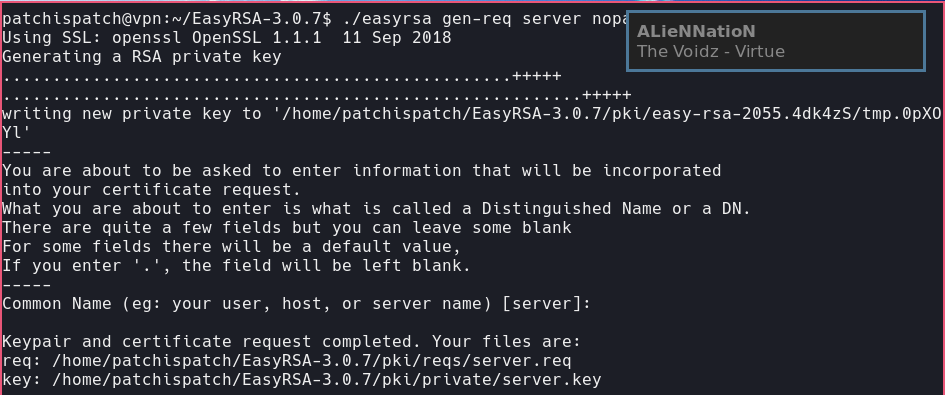
\includegraphics[scale=0.4]{gen-req.png}
\end{center}

\medskip

Esto nos generará una clave privada y el certificado del servidor, llamado \texttt{server.req}. Debemos copiar la clave privada a nuestra carpeta \texttt{/etc/openvpn}. Además, debemos enviar el certificado a nuestro servidor CA. Lo haremos mediante \texttt{scp}:

\medskip

\begin{center}
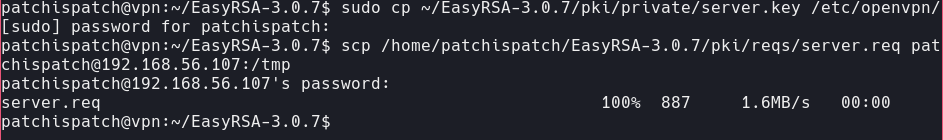
\includegraphics[scale=0.4]{scp-server-req.png}
\end{center}

\medskip

En la máquina CA debemos firmar el certificado con el polivalente script \texttt{easyrsa}. Para importarlo, ejecutamos \texttt{./easyreq import-req /tmp/server.req server}, y para firmarlo utilizamos la opción \texttt{sign-req}:

\medskip

\begin{center}
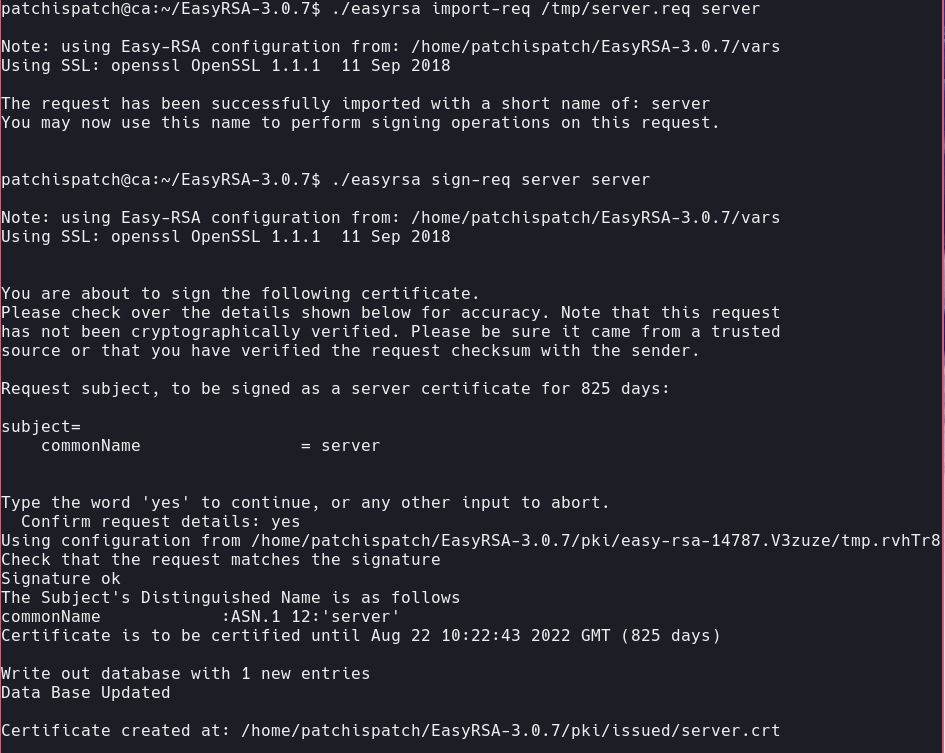
\includegraphics[scale=0.4]{sign-req.png}
\end{center}

\medskip

Ya hemos firmado nuestro certificado, y debemos enviarlo al servidor VPN, de nuevo, utilizando \texttt{scp}. Además, transferimos el certificado de la propia entidad:

\medskip

\texttt{scp pki/issued/server.crt patchispatch@192.168.56.106:/tmp}

\texttt{scp pki/issued/server.crt patchispatch@192.168.56.106:/tmp}

\medskip

Desde la máquina VPN, copiamos los dos certificados a \texttt{/etc/openvpn}.

\medskip

Ahora necesitamos claves de encriptado fuertes, para garantizar la integridad de nuestro servidor VPN. Desde la carpeta EasyRSA-3.0.7 ejecutamos \texttt{./easyrsa gen-dh}, lo que nos generará una clave de cifrado Diffie-Hellman.

\medskip

\begin{center}
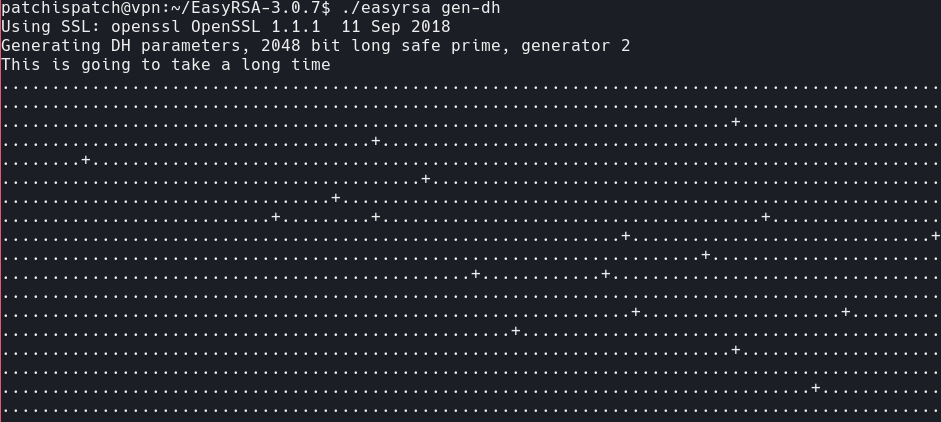
\includegraphics[scale=0.4]{gen-dh.png}
\end{center}

\medskip

Una vez termine el proceso, que en nuestro caso ha tardado alrededor de un minuto, generaremos una firma HMAC con \texttt{openvpn} para fortalecer la seguridad de la verificación aún más:

\medskip

\texttt{openvpn --genkey --secret ta.key}

\medskip

Y cuando termine, copiamos las dos claves a nuestro directorio \texttt{/etc/openvpn}

\medskip

\begin{center}
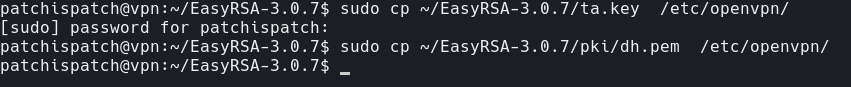
\includegraphics[scale=0.4]{cp-ta-key.png}
\end{center}

\medskip

Ahora disponemos de todas las claves y certificados necesarios para que las máquinas cliente accedan al servidor OpenVPN:

\medskip

\begin{center}
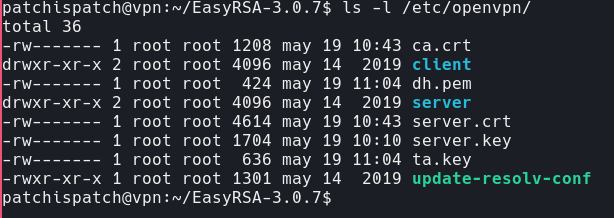
\includegraphics[scale=0.4]{ls-ovpn.png}
\end{center}

\medskip

Para minimizar el riesgo de que accedan a nuestra entidad certificadora, cerramos la sesión. Si la hubiésemos configurado en nuestro servidor vpn, siempre estaría disponible para que un atacante accediese y pudiese firmar certificados ilícitos.

\subsection{Generación del certificado y las claves del cliente}

a generación y firmado de claves se va a realizar desde el servidor, ya que para este ejemplo es más rápido y además permite ser automatizada.

\medskip

Para guardar correctamente los certificados, crearemos la carpeta \texttt{$\sim$/client-configs/keys} en el servidor VPN, y otorgaremos permisos \texttt{700} para asegurarla.

\medskip

Para generar el certificado del primer cliente, al que llamaremos \texttt{client1}, debemos volver al directorio \texttt{EasyRSA-3.0.7}, y ejecutar de nuevo el script con la opción \texttt{gen-req}. También podemos indicar \texttt{nopass} si no queremos contraseña:

\medskip

\texttt{./easyrsa gen-req client1 nopass}

\medskip

\begin{center}
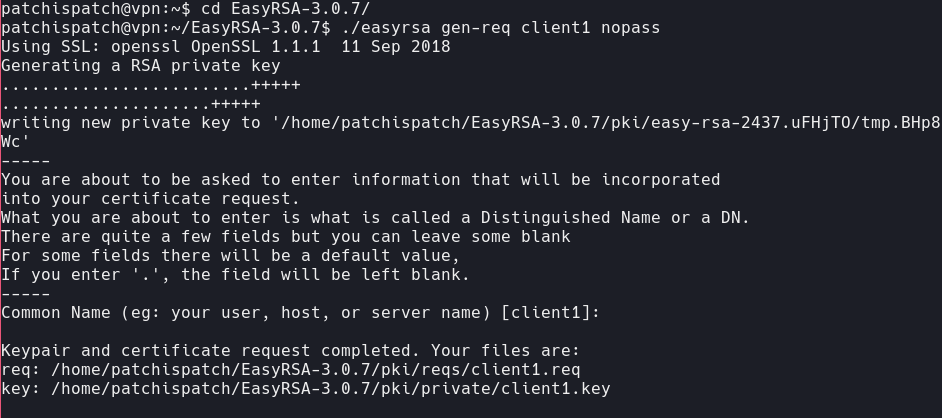
\includegraphics[scale=0.4]{gen-req-client1.png}
\end{center}

\medskip

Copiamos la clave generada a la carpeta creada anteriormente y transferimos el certificado a nuestra máquina CA:

\medskip

\texttt{cp pki/private/client1.key $\sim$/client-configs/keys/}

\texttt{scp pki/reqs/client1.req patchispatch@192.168.56.107:/tmp}

\medskip

En nuestra máquina CA, importamos el certificado como hemos hecho anteriormente, con \texttt{easyrsa import-req}. Una vez hecho esto, procedemos a firmar el certificado, esta vez asegurándonos de que lo hacemos para un cliente:

\medskip

\begin{center}
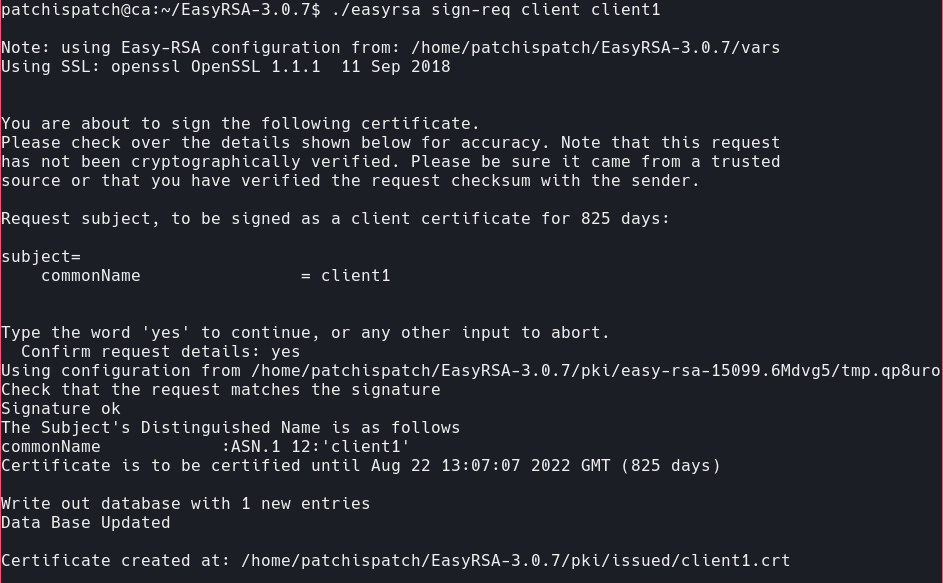
\includegraphics[scale=0.4]{sign-client1.png}
\end{center}

\medskip

Enviamos el certificado firmado al servidor, y una vez allí, lo copiamos a \texttt{$\sim$/client-configs/keys/}. También debemos copiar los archivos \texttt{ta.key} y \texttt{ca.crt} que hemos generado anteriormente.

\medskip

\begin{center}
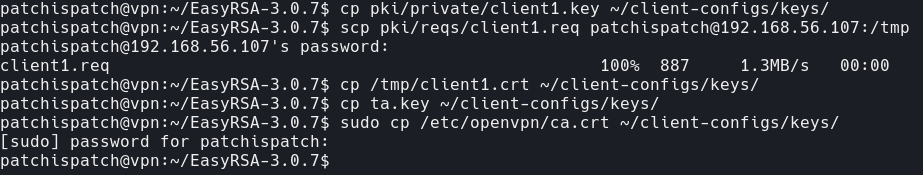
\includegraphics[scale=0.4]{cp-client1.png}
\end{center}

\medskip

Utilizaremos los archivos más adelante. Ahora vamos a configurar el servicio OpenVPN.

\subsection{Configuración del servicio OpenVPN}

\subsubsection{Configuración básica}

Para comenzar a configurar el servicio, copiamos el archivo de configuración de ejemplo:

\medskip

\begin{center}
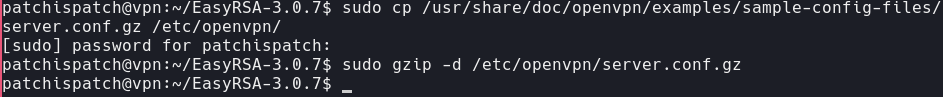
\includegraphics[scale=0.4]{gzip.png}
\end{center}

\medskip

En el archivo de configuración, buscamos la directiva \texttt{tls-auth}. Si la línea en la que se encuentra estuviese comentada, se ha de descomentar. Por lo general, no está comentada por defecto. También debemos descomentar la directiva \texttt{cipher} si no lo estuviera.

\medskip

\begin{center}
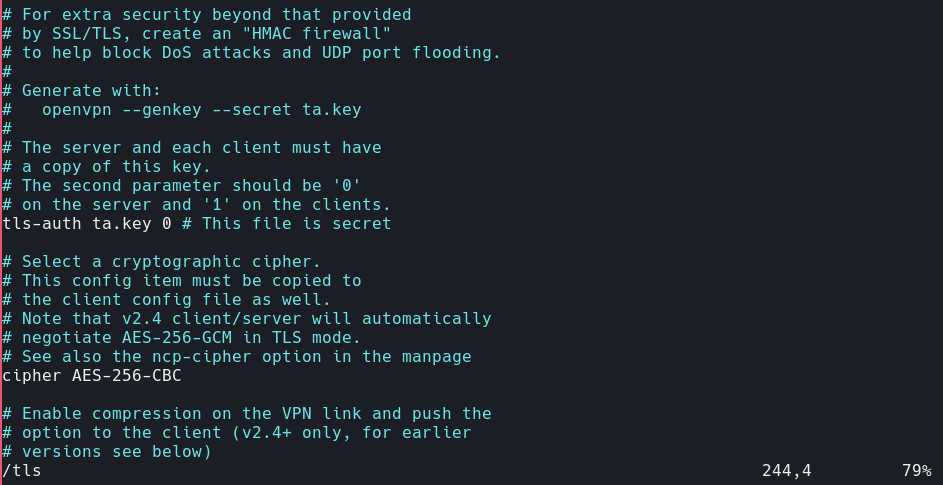
\includegraphics[scale=0.4]{tls-auth.png}
\end{center}

\medskip

Además, debemos añadir debajo de `cipher` la directiva \texttt{auth SHA256}.

\medskip

\begin{center}
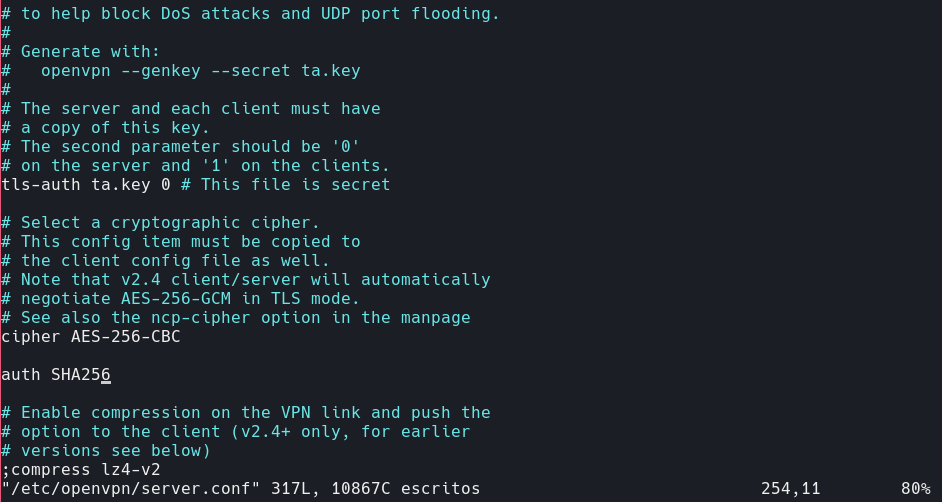
\includegraphics[scale=0.4]{auth-256.png}
\end{center}

\medskip

Debemos buscar también la directiva \texttt{dh}, y cambiar el nombre de archivo para que corresponda con el que generamos anteriormente. En nuestro caso, debemos cambiar \texttt{dh2048.pem} por \texttt{dh.pem}.

\medskip

\begin{center}
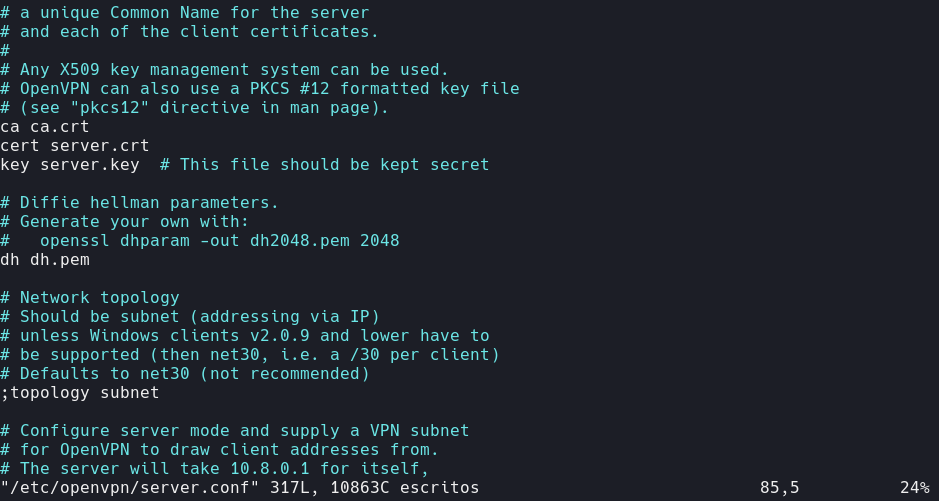
\includegraphics[scale=0.4]{dh-pem.png}
\end{center}

\medskip

Y finalmente descomentamos las líneas de usuario y grupo, ya que estamos utilizando un sistema distinto de Windows.

\medskip

\begin{center}
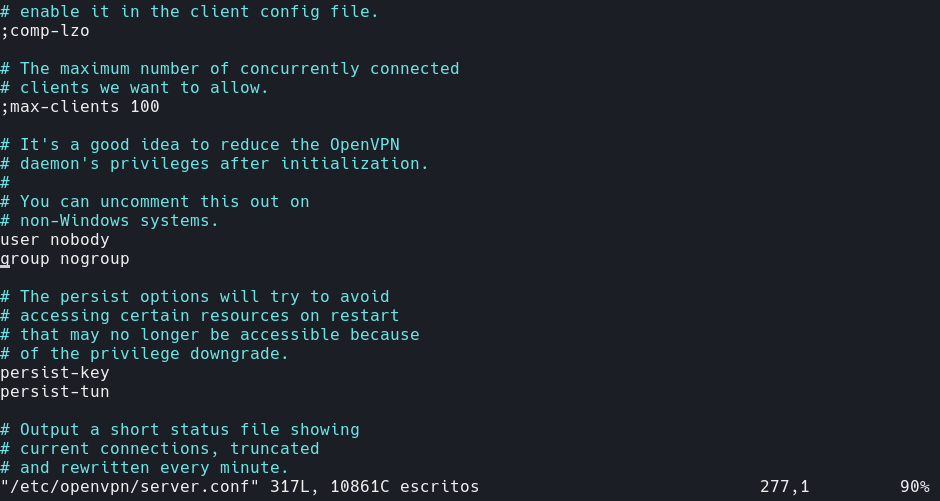
\includegraphics[scale=0.4]{nobody-nogroup.png}
\end{center}

\medskip

\subsubsection{Configuración opcional}

A continuación se van a realizar cambios opcionales en la configuración, detallados en la guía seguida para la instalación. Para las distintas aplicaciones que proponemos sobre cómo utilizar esta tecnología en una granja web serán de mucha utilidad.

\medskip

En concreto, vamos a \textbf{enviar la configuración de DNS a los clientes para que todo el tráfico se redirija a través de la conexión VPN}.

Pese a que con la configuración anterior es suficiente para establecer un túnel, no todo el tráfico tiene por qué atravesarlo. Para conseguir que así sea, debemos modificar algunas partes de la configuración de nuestro servidor.

Como explica la propia configuración, para que todo el tráfico se redirija al túnel VPN se debe habilitar la siguiente opción, borrando el \texttt{;}:

\medskip

\begin{center}
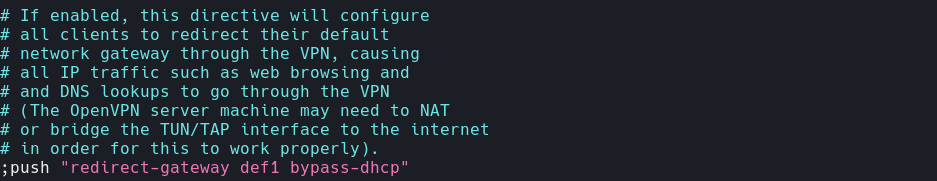
\includegraphics[scale=0.4]{push-redirect.png}
\end{center}

\medskip

También se deben habilitar las dos directivas de debajo para permitir que ciertos tipos de tráfico también pasen por donde queremos:

\medskip

\begin{center}
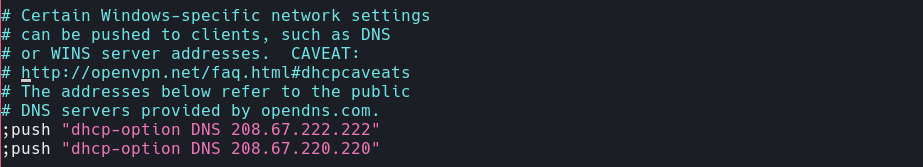
\includegraphics[scale=0.4]{push-dhcp.png}
\end{center}

\medskip

\subsection{Configuración de red del servidor}

Para que nuestra VPN funcione correctamente, debemos habilitar la redirección de IP. Para ello, debemos modificar el archivo \texttt{/etc/sysctl.conf}, y descomentar la siguiente línea:

\medskip

\begin{center}

\includegraphics[scale=0.4]{ipv4-ip.png}
\end{center}

\medskip

Para configurar el enmascaramiento de red, debemos utilizar un firewall. En la instalación hemos utilizado ufw, pero antes de tocar la configuración, debemos identificar la interfaz pública de red ejecutando el siguiente comando: \texttt{ip route | grep default}.

\medskip

\begin{center}

\includegraphics[scale=0.4]{ip-route-grep.png}
\end{center}

\medskip

Nuestra interfaz de red es \texttt{enp0s3}. Ahora debemos modificar el archivo \texttt{before.rules} de la configuración de ufw. Añadimos lo siguiente:

\medskip

\begin{center}
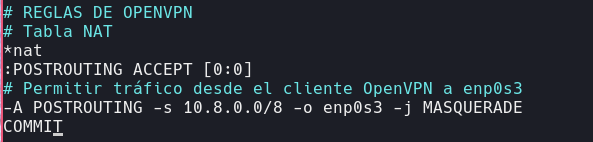
\includegraphics[scale=0.4]{before-rules-vpn.png}
\end{center}

\medskip

Para decirle a ufw que debe permitir paquetes redirigidos, modificamos el archivo \texttt{/etc/default/ufw}, añadiendo la línea siguiente:

\medskip

DEFAULT\_FORWARD\_POLICY=``ACCEPT''

\bigskip

Por último, añadimos las excepciones necesarias para que el firewall permita el tráfico de OpenVPN.

\medskip

OpenVPN utiliza por defecto el puerto 1194 mediante udp. Tanto el puerto como el protocolo pueden modificarse en la configuración, pero nosotros no lo hemos hecho, así que ejecutamos lo siguiente:

\medskip

\begin{center}

\includegraphics[scale=0.4]{ufw-allow-1194.png}
\end{center}

\medskip

Si OpenSSH no estuviese ya listado por ufw, sería necesario añadirlo también. Reiniciamos el servicio y todo estaría listo, al menos en esta parte.

\newpage

\subsection{Iniciar y habilitar el servicio OpenVPN}

Para iniciar el servicio OpenVPN e indicarle que nuestra configuración se halla en el arhivo \texttt{server.conf}, ejecutamos \texttt{sudo systemctl start openvpn@server}. Después, comprobamos su estado:

\medskip

\begin{center}
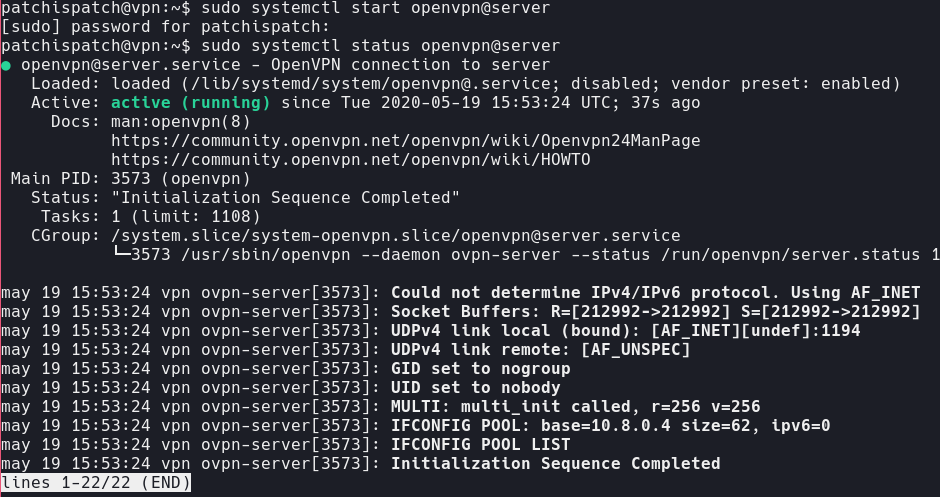
\includegraphics[scale=0.4]{start-openvpn.png}
\end{center}

\medskip

Para que arranque al iniciar, ejecutamos \texttt{sudo systemctl enable openvpn@server}.

Podemos comprobar que se ha creado la interfaz de red de VPN \texttt{tun0}:ç

\medskip

\begin{center}
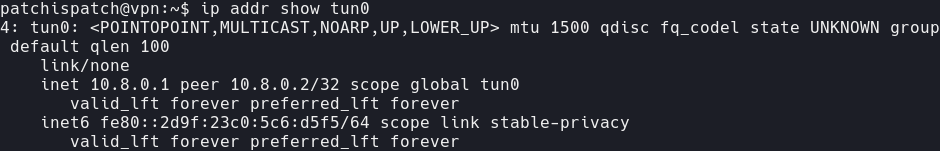
\includegraphics[scale=0.4]{tun0.png}
\end{center}

\medskip

\subsection{Creación de la infraestructura de la configuración de clientes}

La VPN está lista, pero necesitamos configurar los clientes. Dado que cada cliente necesita su configuración personal, vamos a crear una infraestructura para que generar y almacenar las diferentes configuraciones de usuario.

\medskip

Para empezar, creamos la carpeta \texttt{$\sim$/client-configs/files}. Después, copiamos dentro una copia del archivo de configuración de ejemplo proporcionado por OpenVPN, que nos servirá como base.

\medskip

\texttt{\small{cp /usr/share/doc/openvpn/examples/sample-config-files/client.conf $\sim$/client-configs/base.conf}}

\bigskip

Debemos indicar la IP de nuestro servidor OpenVPN, además del puerto, en la directiva \texttt{remote}.

\medskip

\begin{center}
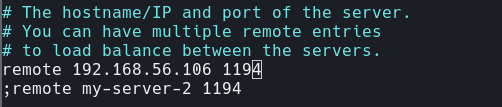
\includegraphics[scale=0.4]{remote.png}
\end{center}

\medskip

Debemos confirmar también que el protocolo seleccionado es UDP, ya que tiene que coincidir con el utilizado por el servidor.

\medskip

\begin{center}
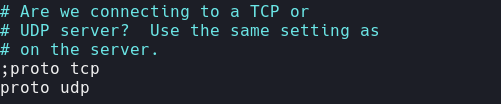
\includegraphics[scale=0.4]{proto-udp.png}
\end{center}

\medskip

De nuevo, descomentamos los campos de usuario y grupo:

\medskip

\begin{center}
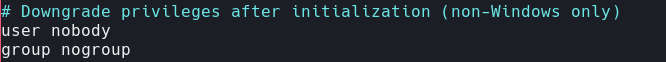
\includegraphics[scale=0.4]{user-client.png}
\end{center}

\medskip

Debemos cambiar la configuración de cifrado tal y como la tenemos en \texttt{/etc/openvpn/server.conf}

\medskip

\begin{center}
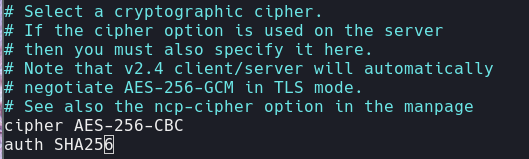
\includegraphics[scale=0.4]{auth-client.png}
\end{center}

\bigskip

Para que la VPN funcione correctamente en el cliente debemos añadir la directiva \texttt{key-direction 1}. Además, vamos a añadir líneas comentadas que puede que necesitemos en los clientes de forma específica.

\medskip

Este primer bloque de instrucciones es para aquellos clientes que \textbf{NO} utilizan \texttt{systemd-resolve} para la gestión de DNS:

\begin{lstlisting}
; script-security 2
; up /etc/openvpn/update-resolv-conf
; down /etc/openvpn/update-resolv-conf
\end{lstlisting}

\medskip

Este es para los que sí lo utilizan:

\begin{lstlisting}
; script-security 2
; up /etc/openvpn/update-systemd-resolved
; down /etc/openvpn/update-systemd-resolved
; down-pre
; dhcp-option DOMAIN-ROUTE .
\end{lstlisting}

\bigskip

Ahora prepararemos un script que automatice la generación de configuracion junto con las claves necesarias, y lo sitúe todo en la carpeta \texttt{client-configs/files}. Abrimos el editor y creamos el script \texttt{make\_config.sh} en la carpeta \texttt{client-configs}:

\medskip

\begin{center}
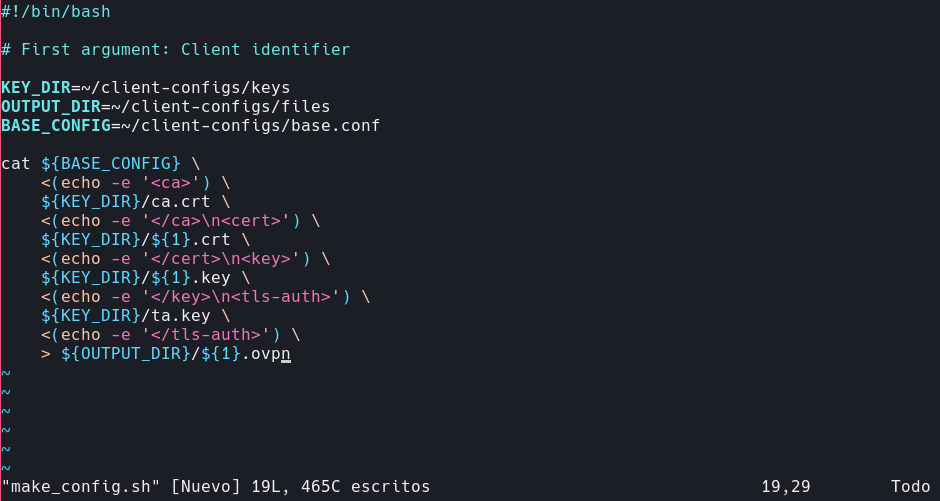
\includegraphics[scale=0.4]{make-config.png}
\end{center}

\medskip

Este script realizará una copia de la configuración base, recogerá los certificados y claves generadas añadiéndolas a la configuración y las colocará en el directorio correspondiente. No obstante, cada vez que se añada un cliente se deberá generar y firmar el certificado correspondiente, algo que vamos a hacer a continuación.

\subsection{Generación de configuración de clientes}

Como tenemos los certificados generados para un cliente llamado \texttt{client1} de un paso anterior, ejecutamos el script. Nos generará un archivo en la carpeta \texttt{files}, llamado \texttt{client1.ovpn}. Este archivo contiene la configuración y será instalado en el cliente.

\medskip

\begin{center}
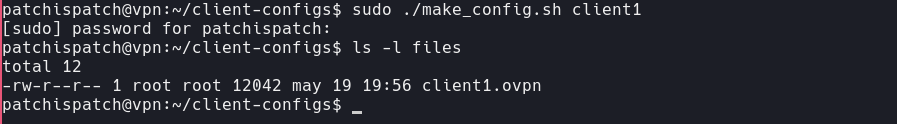
\includegraphics[scale=0.4]{make-config-client1.png}
\end{center}

\bigskip

Debemos transferir este archivo al cliente. Se ha creado una nueva máquina virtual con Ubuntu 18.04 para hacer de cliente de pruebas, llamada \texttt{client} y con IP estática \texttt{192.168.56.108}. 

\medskip

Realizamos la transferencia mediante \texttt{scp}, aunque dependiendo del sistema del cliente tendremos que usar diferentes métodos ---que cubriremos más adelante---, y una vez finalizada tendremos el archivo listo en en la carpeta home de nuestro cliente.

\medskip

\begin{center}
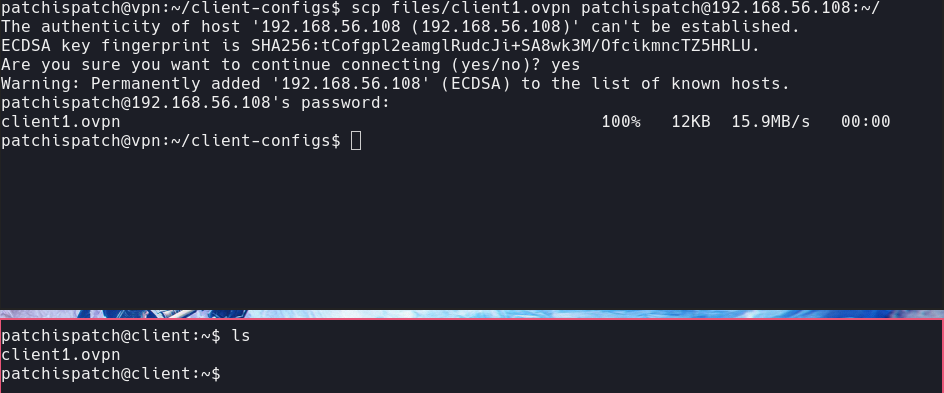
\includegraphics[scale=0.4]{scp-client1.png}
\end{center}

\medskip

\subsection{Instalación de la configuración del cliente}

Dependiendo de las características del cliente, deberemos utilizar diferentes métodos. En este caso realizaremos las pruebas en GNU/Linux y Android.

\subsection{GNU/Linux}

En GNU/Linux, la forma más sencilla y global de configurar el cliente es utilizar el software de OpenVPN. Instalamos con \texttt{sudo apt install openvpn}, como hicimos al principio, ya que estamos utilizando Ubuntu 18.04.

\medskip

Debemos comprobar si nuestro cliente utiliza \texttt{systemd-resolved}. Para ello, comprobamos el archivo \texttt{/etc/resolv.conf}:

\medskip

\begin{center}
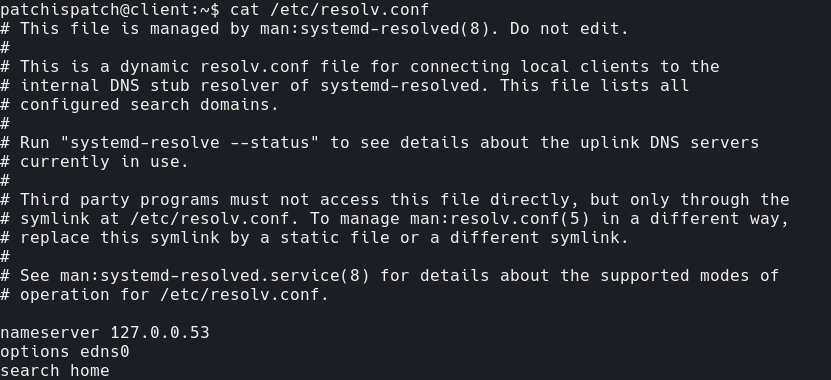
\includegraphics[scale=0.4]{resolv-conf.png}
\end{center}

\medskip

Como la dirección IP que aparece es \texttt{127.0.0.53}, sabemos que nuestro cliente está utilizando \texttt{systemd-resolved}. Para dar soporte a este tipo de clientes, debemos instalar el paquete \texttt{openvpn-systemd-resolved}. De esta forma se forzará al servicio a utilizar la conexión VPN al enviar las resoluciones y consultas DNS.

\medskip

Ahora debemos abrir el archivo de configuración del cliente y descomentar las líneas que añadimos anteriormente correspondientes a systemd-resolved:

\medskip

\begin{center}
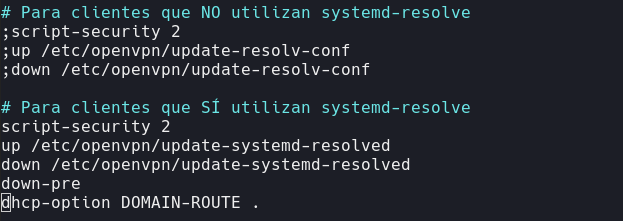
\includegraphics[scale=0.4]{uncomment-systemd-resolved.png}
\end{center}

\medskip

Una vez hecho esto, podemos conectarnos ejecutando \texttt{openvpn} indicando el fichero de configuración.

\medskip

\begin{center}
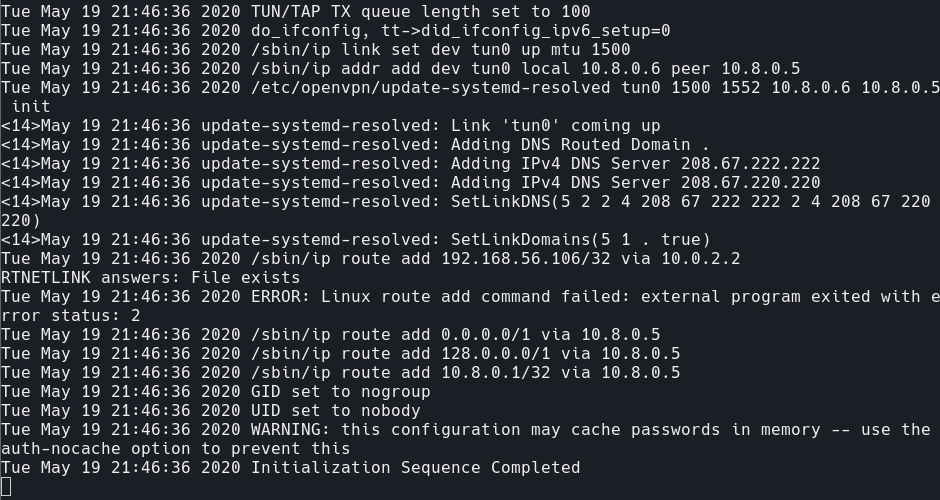
\includegraphics[scale=0.4]{log.png}
\end{center}

\medskip

\subsubsection{Android}

\textit{\textbf{Nota:} para acceder a la VPN desde fuera del host de la máquina virtual y una red distinta, se debe configurar un adaptador puente en la máquina virtual y abrir y configurar los respectivos puertos del router. Para conectarnos desde el móvil en la misma red, basta con configurar un adaptador puente.}

\bigskip

Para empezar, creamos el certificado firmado para un nuevo cliente, \texttt{client2}, siguiendo el procedimiento expuesto en el punto \textbf{\textit{Generación del certificado y las claves del cliente}}.

\medskip

Una vez disponemos del archivo \texttt{client2.ovpn}, debemos configurar el cliente desde nuestro móvil. Para ello, transferimos el archivo, ya sea por USB, ssh o cualquier medio.

\medskip

Descargamos la aplicación \textbf{OpenVPN Connect}, la aplicación oficial de OpenVPN. Una vez tenemos el archivo en nuestro dispositivo, la abrimos y seleccionamos nuestro archivo desde la opción \textit{File}:

\medskip

\begin{center}
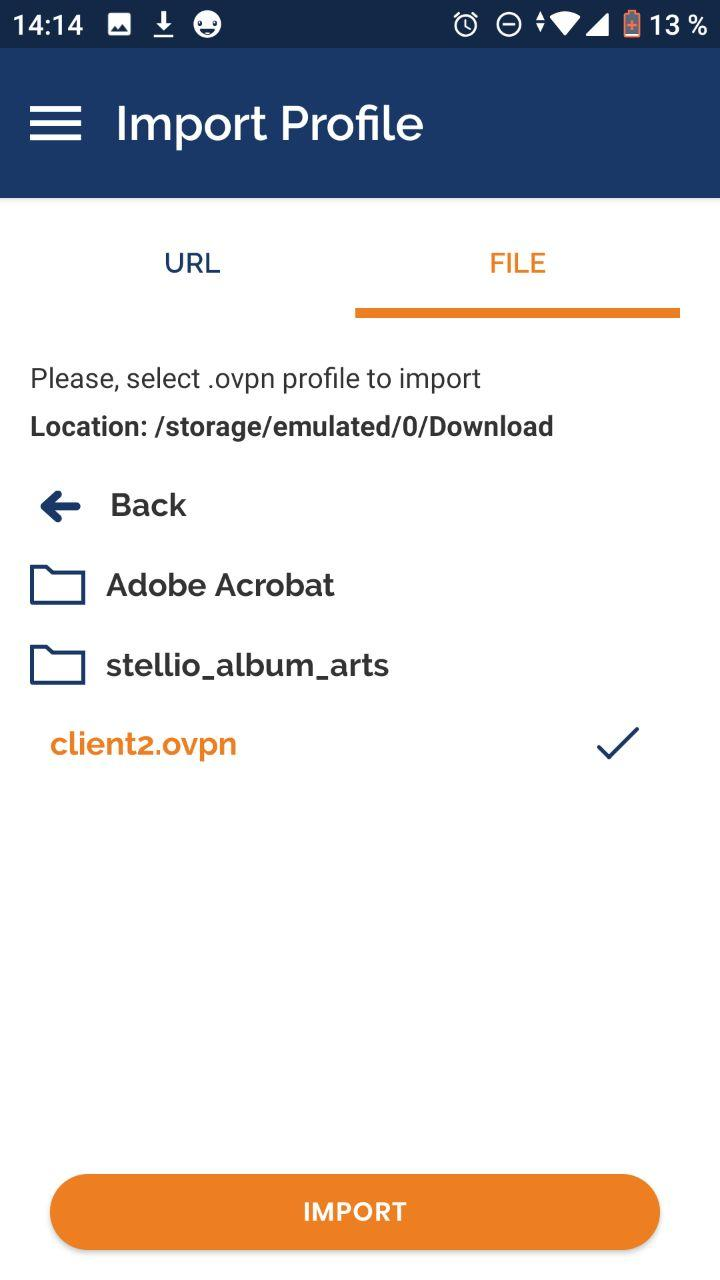
\includegraphics[scale=0.4]{import-profile.jpg}
\end{center}

\medskip

Una vez importado correctamente el perfil podremos cambiar su nombre, y podremos iniciar la conexión. Si todo va bien, la aplicación nos indicará que estamos conectados a nuestra VPN, y aparecerá una notificación mientrar lo sigamos estando.

\medskip

\begin{center}
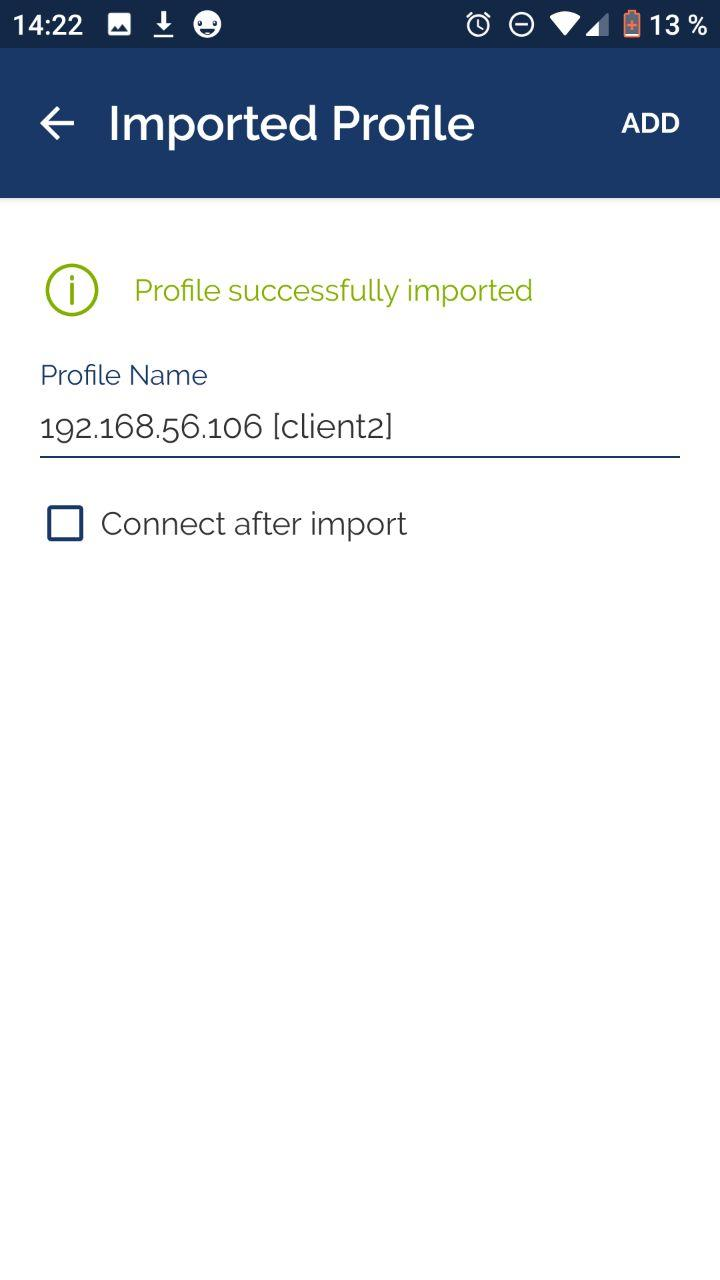
\includegraphics[scale=0.4]{profile-imported.jpg}
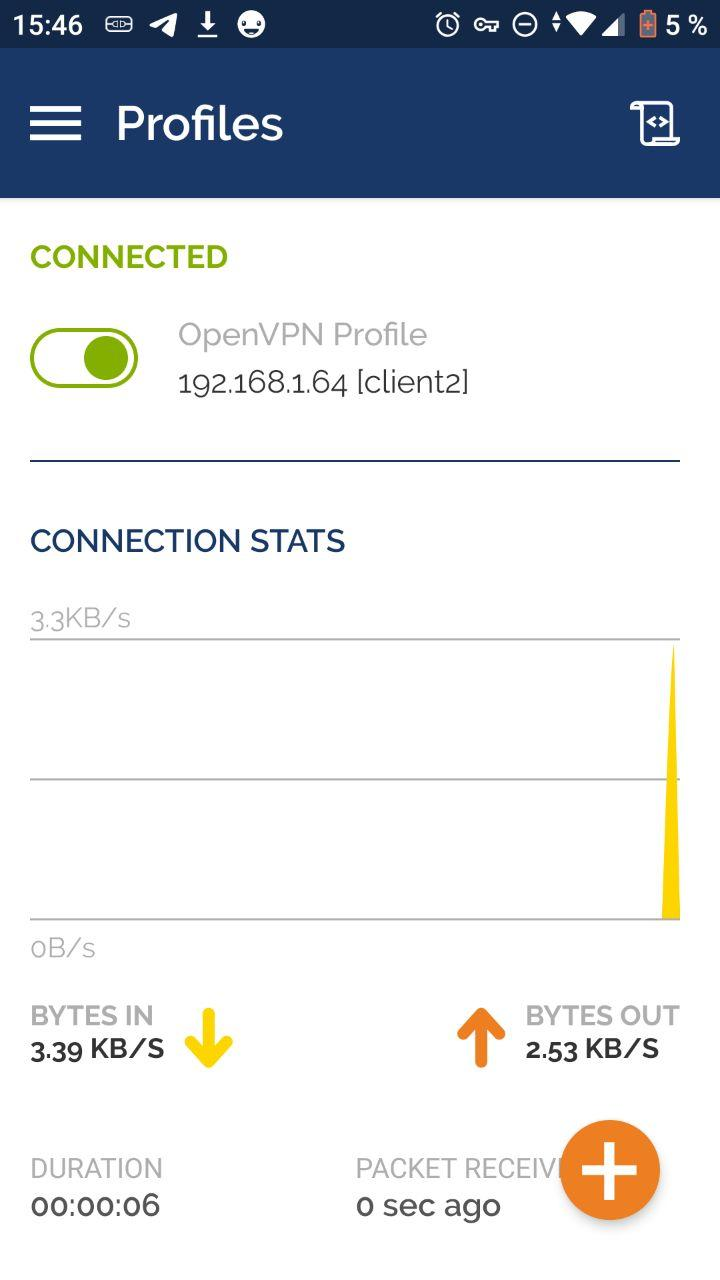
\includegraphics[scale=0.4]{connected.jpg}
\end{center}

\newpage

\section{Aplicaciones a centros de datos y seguridad}

El proceso de instalación y configuración del servicio ya está terminado, y nos da una idea de cómo proceder a la hora de utilizarlo de forma relativamente sencilla. La tecnología VPN ofrece una serie de características que pueden ser muy útiles en granjas de servidores. Exploraremos dos usos diferentes para esta tecnología:

\subsection{Uso 1: asegurar el acceso remoto a una granja web}

Ya sea por tratarse de una red interna de trabajo o por cuestiones de mantenimiento, se puede utilizar una conexión VPN y un firewall para limitar quién puede acceder a las diferentes máquinas de nuestro centro de datos físico.

\medskip

Permitiendo acceso únicamente a través del túnel VPN para ciertos servicios como por ejemplo SSH, podemos distribuir certificados a los distintos encargados de mantenimiento de nuestros servidores de contenido, permitiendo así una gestión más cómoda sin comprometer la seguridad de nuestra granja.

\medskip

Podemos limitar el acceso de diferentes maneras:

\subsubsection*{Limitar el acceso a toda la red}

Esta configuración es útil cuando queremos establecer una red de trabajo distribuida y permitir el acceso a empleados y miembros de la institución. La UGR utiliza esta configuración para varios de sus servicios, como el \textit{acortador de URLs} o el servidor Turing de la ETSIIT, a los que se puede acceder únicamente desde la red de la universidad. Si no se dispone de conexión a eduroam, se puede acceder a través de la VPN de la UGR.

\subsubsection*{Limitar el acceso a los servidores de contenido}

Esta configuración no restringe el acceso al balanceador de carga, y permite que se sirvan los contenidos deseados a cualquier usuario, pero para facilitar el mantenimiento si hay algún error o se desea modificar algo de los servidores de contenido de forma remota se puede establecer acceso mediante SSH por VPN. 

\medskip

De esta forma no es necesario mantener un registro de las diferentes IPs de los trabajadores en las reglas del firewall para poder acceder, únicamente es necesario poseer el certificado correspondiente. Hemos visto que generar certificados es sencillo y automatizable, por lo que de cara a conceder acceso supone una opción más cómoda que modificar la configuración del firewall de cada máquina, y a la hora de revocar permisos basta con anular el certificado, algo que también es sencillo.

\subsection{Uso 2: construir un centro de datos de forma distribuida}

La tecnología VPN permite en esencia recrear una red local de forma distribuida, así que podemos utilizar esto para construir un centro de datos y asegurar las transferencias de información entre servidores.

\medskip

Al estar las comunicaciones cifradas, los ataques \textit{man in the middle} no suponen un problema, pero hay que tener en cuenta que el tráfico pasará por el servidor VPN, pudiendo saturarse o fallar, y condicionando el estado de la red entera. Para evitar esto se debe proporcionar una infraestructura más compleja, con varios servidores VPN.

\medskip

El acceso también estaría restringido gracias a los certificados, siempre y cuando configuremos debidamente los servidores y sus respectivos cortafuegos. No todo el tráfico tiene por qué pasar por el túnel VPN, y se puede permitir el acceso desde fuera de la red privada a diferentes protocolos y servicios, como HTTPS en el balanceador de carga. 

\medskip

OpenVPN es bastante flexible en cuanto a la configuración se refiere, por lo que se podría aplicar, por ejemplo, a proteger la duplicación de datos y el acceso a los servidores de contenido, dejando libre el tráfico de datos menos sensibles para no saturar el túnel.

\section{Conclusión}

La tecnología VPN es mucho más flexible de lo que esperaba encontrar en un principio, y dado que ahora está pasando por una nueva etapa de popularidad debido a los servicios de suscripción y poder cambiar tu identidad en línea, me llamaba la atención explorar cómo podía aplicarse a los contenidos de la asignatura. Que la instalación requiera editar archivos de configuración de red y construir una entidad certificadora SSL me ha parecido muy formativo, y la gran cantidad de opciones de las que dispone el servicio OpenVPN, así como su capacidad multiplataforma y gran comunidad y documentación, han ayudado a comprender mejor los posibles usos de esta herramienta.

\newpage

\section{Bibliografía}

\url{https://www.digitalocean.com/community/tutorials/initial-server-setup-with-ubuntu-18-04}

\url{https://www.digitalocean.com/community/tutorials/how-to-set-up-an-openvpn-server-on-ubuntu-18-04}

\url{https://askubuntu.com/questions/920486/openvpn-config-client-ovpn-fail-rtnetlink-answers-file-exists}

\url{https://community.openvpn.net/openvpn/wiki}

\url{https://openvpn.net/community-resources/configuring-client-specific-rules-and-access-policies/}

\url{https://openvpn.net/community-resources/ethernet-bridging/}

\url{https://openvpn.net/community-resources/installing-openvpn/}

\url{https://openvpn.net/community-resources/setting-up-your-own-certificate-authority-ca/}

\end{document}